% !TEX program = xelatex
\documentclass[aspectratio=169,11pt]{beamer}

\usepackage{fontspec}
\setsansfont{Arial}
\setmainfont{Times New Roman}
\usepackage{graphicx}
\usepackage{booktabs}
\usepackage{tabularx}
\usepackage{amsmath}
\usepackage{tikz}
\usetikzlibrary{positioning,arrows.meta}
\usepackage{xcolor}

\definecolor{sgublue}{RGB}{0,51,102}
\definecolor{sgulight}{RGB}{235,242,250}
\definecolor{sgugray}{RGB}{90,90,90}

\usetheme{Madrid}
\usecolortheme{default}
\setbeamertemplate{navigation symbols}{}
\setbeamertemplate{headline}{}
\setbeamercolor{structure}{fg=sgublue}
\setbeamercolor{frametitle}{bg=sgublue,fg=white}
\setbeamerfont{frametitle}{size=\large,series=\bfseries}
\setbeamercolor{title}{fg=sgublue}
\setbeamercolor{author}{fg=sgugray}
\setbeamercolor{institute}{fg=sgugray}
\setbeamercolor{block title}{bg=sgulight,fg=sgublue}
\setbeamercolor{block body}{bg=sgulight!40}
\setbeamertemplate{itemize items}[circle]
\setbeamertemplate{enumerate items}[default]
\setbeamertemplate{blocks}[rounded][shadow=false]
\setbeamertemplate{footline}{
  \leavevmode
  \hbox{
    \begin{beamercolorbox}[wd=.33\paperwidth,ht=2.4ex,dp=1ex,center]{author in head/foot}
      \usebeamerfont{author in head/foot}\insertshortauthor
    \end{beamercolorbox}
    \begin{beamercolorbox}[wd=.41\paperwidth,ht=2.4ex,dp=1ex,center]{title in head/foot}
      \usebeamerfont{title in head/foot}\insertshorttitle
    \end{beamercolorbox}
    \begin{beamercolorbox}[wd=.24\paperwidth,ht=2.4ex,dp=1ex,right]{date in head/foot}
      \usebeamerfont{date in head/foot}\insertframenumber/\inserttotalframenumber
    \end{beamercolorbox}
  }
}

\newcommand{\good}[1]{\textcolor{sgublue}{\textbf{#1}}}
\newcommand{\bad}[1]{\textcolor{red!70!black}{\textbf{#1}}}

\title[Multi-task UIT-VSFC]{Multi-task Learning cho Phân loại Cảm xúc và Chủ đề Phản hồi Sinh viên Tiếng Việt}
\subtitle{So sánh TextCNN và PhoBERT}
\author[Đinh Quang Minh]{Đinh Quang Minh (3123580024) -- Nhóm trưởng\\Dương Tấn Cường (3123580004)\\Lê Thành Duy (3123580007)}
\institute[ĐH Sài Gòn]{Trường Đại học Sài Gòn -- Khoa Toán - Ứng dụng\\Giảng viên hướng dẫn: TS. Trịnh Tấn Đạt\\Môn: Lập trình Python nâng cao (858043)}
\date{Tháng 11 năm 2026}

\begin{document}

% ==================== 1. BÌA ====================
\begin{frame}[plain]
\begin{tikzpicture}[remember picture, overlay]
  \draw[line width=1.1pt, color=sgublue]
    ([xshift=0.38cm,yshift=-0.38cm]current page.north west)
    rectangle
    ([xshift=-0.38cm,yshift=0.38cm]current page.south east);
  \draw[line width=0.35pt, color=sgublue]
    ([xshift=0.50cm,yshift=-0.50cm]current page.north west)
    rectangle
    ([xshift=-0.50cm,yshift=0.50cm]current page.south east);
\end{tikzpicture}
\begin{center}
\vspace*{-0.15cm}
{\scriptsize\bfseries ỦY BAN NHÂN DÂN THÀNH PHỐ HỒ CHÍ MINH}\\[0.02cm]
{\small\bfseries TRƯỜNG ĐẠI HỌC SÀI GÒN}\\[0.01cm]
{\scriptsize\bfseries KHOA TOÁN - ỨNG DỤNG}\\[0.06cm]

\includegraphics[width=1.35cm]{../reports/SGU-LOGO.png}\\[0.05cm]
{\scriptsize BÁO CÁO GIỮA KÌ}\\[0.07cm]
{\large\bfseries Multi-task Learning cho Phân loại Cảm xúc\\
và Chủ đề Phản hồi Sinh viên Tiếng Việt}\\[0.05cm]
{\small So sánh TextCNN và PhoBERT}\\[0.10cm]
{\scriptsize Ngành: Khoa học dữ liệu \quad|\quad Môn: Lập trình Python nâng cao (858043)}\\[0.04cm]
{\scriptsize GVHD: TS. Trịnh Tấn Đạt}\\[0.06cm]
{\scriptsize
Đinh Quang Minh (3123580024) -- Nhóm trưởng\\
Dương Tấn Cường (3123580004)\\
Lê Thành Duy (3123580007)}\\[0.07cm]
{\scriptsize Thành phố Hồ Chí Minh, tháng 11 năm 2026}
\end{center}
\end{frame}

% ==================== 2. PHẦN 1 ====================
\begin{frame}[plain]
\begin{center}
\vspace*{0.9cm}
{\small\bfseries\color{sgublue} PHẦN 1}\\[0.25cm]
{\Huge\bfseries\color{sgublue} BÀI TOÁN \& SẢN PHẨM}\\[0.2cm]
{\color{sgublue}\rule{0.55\textwidth}{0.8pt}}\\[0.2cm]
{\large Trình bày: Đinh Quang Minh}\\[0.2cm]
{\small Bài toán, mục tiêu, pipeline, demo}\\[0.15cm]
\end{center}
\end{frame}

% ==================== 5. BÀI TOÁN ====================
\begin{frame}{Bài toán và động lực}
\begin{columns}[T]
\begin{column}{0.55\textwidth}
\textbf{Đầu vào:} một câu phản hồi sinh viên tiếng Việt.

\vspace{0.25cm}
\textbf{Đầu ra:}
\begin{itemize}
  \item Cảm xúc: tiêu cực / trung tính / tích cực.
  \item Chủ đề: giảng viên / chương trình / cơ sở vật chất / khác.
\end{itemize}

\vspace{0.25cm}
\textbf{Vì sao cần?}
\begin{itemize}
  \item Phản hồi nhiều, đọc thủ công tốn thời gian.
  \item Chỉ biết ``có vấn đề'' là chưa đủ; cần biết \emph{vấn đề ở đâu}.
  \item Cần tín hiệu có thể hành động, không chỉ một nhãn.
\end{itemize}
\end{column}
\begin{column}{0.42\textwidth}
\begin{block}{Ví dụ}
\textit{``Thầy dạy nhiệt tình nhưng phòng học thiếu máy chiếu.''}

\vspace{0.2cm}
$\Rightarrow$ positive + lecturer\\
$\Rightarrow$ negative + facility
\end{block}

\vspace{0.2cm}
\begin{alertblock}{Điểm khó}
Câu thực tế thường có nhiều chủ đề; nhãn hiện tại chỉ là single-label.
\end{alertblock}
\end{column}
\end{columns}
\end{frame}

% ==================== 6. MỤC TIÊU ====================
\begin{frame}{Mục tiêu và đóng góp}
\begin{columns}[T]
\begin{column}{0.48\textwidth}
\textbf{Mục tiêu}
\begin{itemize}
  \item Pipeline tái lập cho UIT-VSFC.
  \item So sánh TextCNN và PhoBERT.
  \item Cải thiện topic head bằng keyword.
  \item Đánh giá 3 seed + kiểm định.
  \item Nén mô hình để chạy CPU.
  \item Demo có calibration và cảnh báo.
\end{itemize}
\end{column}
\begin{column}{0.48\textwidth}
\textbf{Đóng góp}
\begin{itemize}
  \item TextCNN multi-task và PhoBERT frozen.
  \item Keyword-aware + auxiliary loss.
  \item 3 seed, McNemar, bootstrap.
  \item TextCNN student distilled.
  \item Calibration + robustness.
  \item Demo Streamlit có top-2 và multi-topic warning.
\end{itemize}
\end{column}
\end{columns}

\vspace{0.25cm}
\begin{block}{Câu hỏi xuyên suốt}
Mô hình nào tốt hơn, cải thiện có bền vững không, và có thể triển khai trên CPU không?
\end{block}
\end{frame}

% ==================== 7. PIPELINE ====================
\begin{frame}{Pipeline tổng quan}
\begin{center}
\resizebox{0.95\textwidth}{!}{%
\begin{tikzpicture}[
  node distance=0.9cm,
  box/.style={draw=sgublue, fill=sgulight, rounded corners, minimum width=2.4cm, minimum height=0.8cm, align=center},
  arr/.style={-{Latex[length=2mm]}, thick, color=sgublue}
]
\node[box] (data) {UIT-VSFC};
\node[box, right=of data] (pre) {Tiền xử lý\\Unicode + tách từ};
\node[box, right=of pre] (enc) {Encoder\\TextCNN / PhoBERT};
\node[box, right=of enc, yshift=0.8cm] (sent) {Sentiment head};
\node[box, right=of enc, yshift=-0.8cm] (topic) {Topic head};
\node[box, right=of sent] (out_s) {Cảm xúc};
\node[box, right=of topic] (out) {Chủ đề};
\draw[arr] (data) -- (pre);
\draw[arr] (pre) -- (enc);
\draw[arr] (enc) -- (sent);
\draw[arr] (enc) -- (topic);
\draw[arr] (sent) -- (out_s);
\draw[arr] (topic) -- (out);
\node[box, below=0.8cm of enc, dashed] (kw) {12 keyword features};
\draw[arr, dashed] (kw) -- (topic);
\end{tikzpicture}}
\end{center}

\vspace{0.1cm}
\begin{columns}[T]
\begin{column}{0.32\textwidth}
\begin{block}{Dữ liệu}
Train 11.426 / dev 1.583 / test 3.166.
\end{block}
\end{column}
\begin{column}{0.32\textwidth}
\begin{block}{Hai task}
Một encoder, hai head, một lần suy luận.
\end{block}
\end{column}
\begin{column}{0.32\textwidth}
\begin{block}{Triển khai}
Teacher PhoBERT $\rightarrow$ student TextCNN.
\end{block}
\end{column}
\end{columns}
\end{frame}

% ==================== 8. DEMO ====================
\begin{frame}{Demo Streamlit và ý nghĩa thực tế}
\begin{columns}[T]
\begin{column}{0.48\textwidth}
\textbf{ Demo có gì?}
\begin{itemize}
  \item Chọn teacher / student.
  \item Confidence đã calibration.
  \item Top-2 chủ đề.
  \item Keyword chủ đề phát hiện.
  \item Latency và số tham số.
  \item Cảnh báo multi-topic.
\end{itemize}
\end{column}
\begin{column}{0.48\textwidth}
\begin{block}{Triage phản hồi}
\begin{tabular}{@{}ll@{}}
\toprule
Cặp & Hành động gợi ý \\
\midrule
negative + lecturer & Xem lại giảng dạy \\
negative + facility & Kiểm tra phòng/thiết bị \\
negative + training & Xem lại chương trình \\
positive + lecturer & Ghi nhận, nhân rộng \\
\bottomrule
\end{tabular}
\end{block}
\end{column}
\end{columns}

\vspace{0.2cm}
\begin{block}{Thông điệp}
Hệ thống là công cụ \emph{hỗ trợ} đọc và ưu tiên phản hồi, không thay thế con người.
\end{block}
\end{frame}

% ==================== 9. PHẦN 2 ====================
\begin{frame}[plain]
\begin{center}
\vspace*{0.9cm}
{\small\bfseries\color{sgublue} PHẦN 2}\\[0.25cm]
{\Huge\bfseries\color{sgublue} DỮ LIỆU, MÔ HÌNH \& ĐỘ TIN CẬY}\\[0.2cm]
{\color{sgublue}\rule{0.55\textwidth}{0.8pt}}\\[0.2cm]
{\large Trình bày: Dương Tấn Cường}\\[0.2cm]
{\small UIT-VSFC, EDA, TextCNN, PhoBERT, calibration, robustness}\\[0.15cm]
\end{center}
\end{frame}

% ==================== 10. DATASET ====================
\begin{frame}{UIT-VSFC: dữ liệu và nhãn}
\begin{columns}[T]
\begin{column}{0.44\textwidth}
\textbf{Quy mô}
\vspace{0.15cm}
\begin{tabular}{@{}lr@{}}
\toprule
Split & Số câu \\
\midrule
Train & 11.426 \\
Dev & 1.583 \\
Test & 3.166 \\
\midrule
Tổng & 16.175 \\
\bottomrule
\end{tabular}

\vspace{0.45cm}
\textbf{Nhãn}
\begin{itemize}
  \item Sentiment: negative, neutral, positive.
  \item Topic: lecturer, training\_program, facility, others.
\end{itemize}
\end{column}
\begin{column}{0.52\textwidth}
\begin{block}{Vì sao dùng macro-F1?}
\begin{itemize}
  \item \texttt{neutral} chỉ khoảng 4.0\% train.
  \item \texttt{lecturer} khoảng 71.5\% train.
  \item Accuracy dễ bị chi phối bởi lớp đa số.
\end{itemize}
\end{block}

\begin{alertblock}{Lưu ý}
Nhãn topic là nhãn mức câu, không phải aspect. Một câu nhiều chủ đề vẫn chỉ có một nhãn.
\end{alertblock}
\end{column}
\end{columns}
\end{frame}

% ==================== 11. EDA ====================
\begin{frame}{EDA: những con số định hướng thiết kế}
\begin{columns}[T]
\begin{column}{0.55\textwidth}
\begin{itemize}
  \item p95 độ dài câu train: \good{33 token} $\Rightarrow$ chọn \texttt{max\_len=48}.
  \item \texttt{neutral} chỉ \good{4.0\%} train.
  \item \texttt{lecturer} chiếm \good{71.5\%} train.
  \item \texttt{facility} gần như luôn tiêu cực: \good{474/497} câu.
  \item Không có trùng lặp giữa train/dev/test; 1 câu trùng nội bộ trong train.
\end{itemize}

\vspace{0.25cm}
\begin{block}{Hệ quả}
Dùng class weight, macro-F1, per-class analysis; cẩn thận shortcut ``facility = negative''.
\end{block}
\end{column}
\begin{column}{0.42\textwidth}
\centering
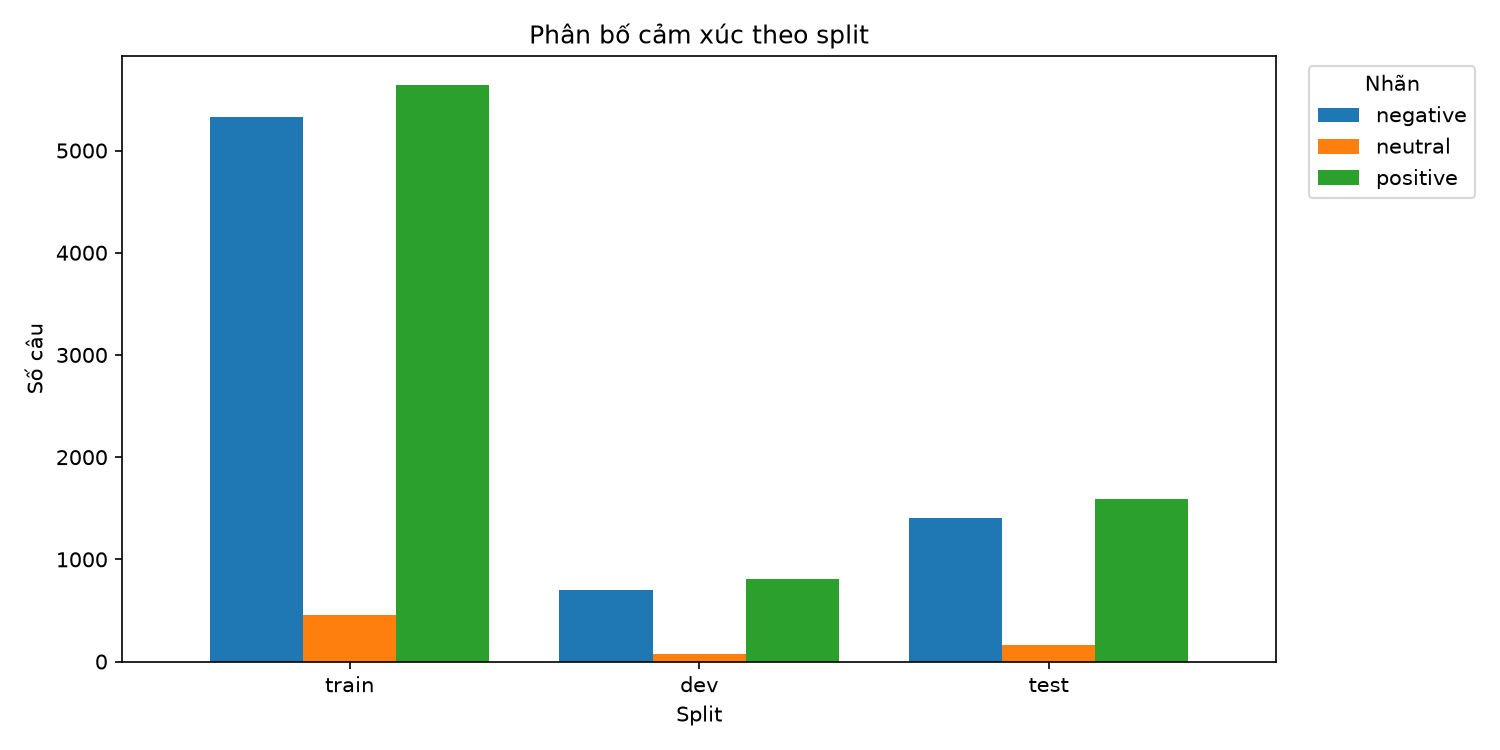
\includegraphics[width=\textwidth]{../reports/data/figures/sentiment_distribution.png}\\
{\scriptsize Phân bố cảm xúc trong train}
\end{column}
\end{columns}
\end{frame}

% ==================== 12. MULTI-TASK ====================
\begin{frame}{Multi-task learning}
\begin{columns}[T]
\begin{column}{0.5\textwidth}
\textbf{Một encoder, hai head}
\[
\mathcal{L} = \mathcal{L}_s + \lambda_t \mathcal{L}_t
\]
\begin{itemize}
  \item $\mathcal{L}_s$: cross-entropy sentiment.
  \item $\mathcal{L}_t$: cross-entropy topic.
  \item $\lambda_t$: điều chỉnh ảnh hưởng của topic.
\end{itemize}

\vspace{0.2cm}
\begin{block}{Kỳ vọng}
Chia sẻ biểu diễn giúp học tốt hơn khi dữ liệu nhỏ; một lần suy luận cho hai output.
\end{block}
\end{column}
\begin{column}{0.46\textwidth}
\begin{block}{Rủi ro}
\textbf{Negative transfer}: task này kéo lùi task kia nếu phân bố/độ khó khác nhau.
\end{block}

\vspace{0.2cm}
\textbf{Cách kiểm tra}
\begin{itemize}
  \item So TextCNN single vs multi.
  \item So PhoBERT frozen vs keyword.
  \item 3 seed + kiểm định.
\end{itemize}
\end{column}
\end{columns}
\end{frame}

% ==================== 13. TEXTCNN ====================
\begin{frame}{TextCNN: nhẹ, nhanh, phù hợp CPU}
\begin{columns}[T]
\begin{column}{0.55\textwidth}
\begin{itemize}
  \item Embedding 100 chiều.
  \item Convolution 1D với kernel 3, 4, 5.
  \item 100 filter mỗi kernel; max-pooling.
  \item Shared hidden 256; dropout 0.5.
  \item Hai head tuyến tính.
  \item Khoảng \good{0.41 triệu} tham số.
\end{itemize}
\end{column}
\begin{column}{0.42\textwidth}
\begin{block}{Ưu điểm}
\begin{itemize}
  \item Train từ đầu, không cần GPU.
  \item Bắt n-gram cục bộ tốt.
  \item Inference rất nhanh.
\end{itemize}
\end{block}
\begin{alertblock}{Hạn chế}
Không mô hình hóa ngữ cảnh xa; phụ thuộc embedding và dữ liệu train.
\end{alertblock}
\end{column}
\end{columns}
\end{frame}

% ==================== 14. PHOBERT + KEYWORD ====================
\begin{frame}{PhoBERT frozen và keyword-aware head}
\begin{columns}[T]
\begin{column}{0.48\textwidth}
\textbf{PhoBERT frozen}
\begin{itemize}
  \item Encoder \texttt{vinai/phobert-base} đóng băng.
  \item Lấy \texttt{[CLS]} 768 chiều.
  \item Shared 256 $\rightarrow$ hai head.
  \item Chỉ train head: \good{18--22 giây}.
  \item Khoảng 135 triệu tham số.
\end{itemize}
\end{column}
\begin{column}{0.48\textwidth}
\textbf{Keyword-aware}
\begin{itemize}
  \item 12 đặc trưng: presence, density, last-3 cho 4 topic.
  \item Topic head nhận thêm vector keyword.
  \item Auxiliary loss $\beta=0.5$.
  \item Class weight \texttt{sqrt\_balanced}.
\end{itemize}
\[
\mathcal{L} = \mathcal{L}_s + \lambda_t\mathcal{L}_t + \beta\mathcal{L}_{kw}
\]
\end{column}
\end{columns}

\vspace{0.15cm}
\begin{block}{Kết quả then chốt}
Keyword-aware tăng topic \good{+0.0205} và joint \good{+0.0199} so với PhoBERT frozen (seed 42).
\end{block}
\end{frame}

% ==================== 15. CALIBRATION ====================
\begin{frame}{Calibration: confidence có đáng tin?}
\small
\begin{center}
\begin{tabular}{@{}llrrr@{}}
\toprule
Model & Task & T & ECE trước & ECE sau \\
\midrule
Teacher & sentiment & 1.366 & 0.0242 & 0.0215 \\
Teacher & topic & 1.230 & 0.0254 & \good{0.0097} \\
Student & sentiment & 1.930 & 0.0658 & \good{0.0166} \\
Student & topic & 1.823 & 0.0805 & \good{0.0145} \\
\bottomrule
\end{tabular}
\end{center}

\vspace{0.2cm}
\begin{columns}[T]
\begin{column}{0.55\textwidth}
\begin{itemize}
  \item Student overconfident hơn teacher trước calibration.
  \item Temperature scaling giảm ECE mạnh.
  \item Accuracy không đổi: chỉ sửa confidence, không sửa nhãn.
\end{itemize}
\end{column}
\begin{column}{0.42\textwidth}
\begin{block}{Cách làm}
Fit temperature trên dev, đánh giá ECE trên test với 15 bins.
\end{block}
\end{column}
\end{columns}
\end{frame}

% ==================== 16. ROBUSTNESS ====================
\begin{frame}{Robustness: mô hình yếu ở đâu?}
\small
\begin{columns}[T]
\begin{column}{0.52\textwidth}
\begin{tabular}{@{}lrr@{}}
\toprule
Variant & Teacher & Student \\
\midrule
Clean & 0.7727 & 0.7322 \\
Không dấu & \bad{0.1517} & \bad{0.1165} \\
Teencode & 0.6833 & 0.6303 \\
Typo & 0.7699 & 0.7005 \\
Emoji & 0.6661 & \good{0.7440} \\
Đảo trật tự & 0.6678 & \good{0.7099} \\
\bottomrule
\end{tabular}
\end{column}
\begin{column}{0.45\textwidth}
\begin{block}{Nhận xét}
\begin{itemize}
  \item Mất dấu là điểm yếu nghiêm trọng nhất.
  \item Teacher nhạy với emoji và shuffle.
  \item Student bền vững hơn ở hai perturbation này.
\end{itemize}
\end{block}
\end{column}
\end{columns}

\vspace{0.15cm}
\begin{alertblock}{Hàm ý}
Cần chuẩn hóa input và bổ sung augmentation trước khi triển khai thực tế.
\end{alertblock}
\end{frame}

% ==================== 17. PHẦN 3 ====================
\begin{frame}[plain]
\begin{center}
\vspace*{0.9cm}
{\small\bfseries\color{sgublue} PHẦN 3}\\[0.25cm]
{\LARGE\bfseries\color{sgublue} THỰC NGHIỆM, KẾT QUẢ \& KẾT LUẬN}\\[0.2cm]
{\color{sgublue}\rule{0.55\textwidth}{0.8pt}}\\[0.2cm]
{\large Trình bày: Lê Thành Duy}\\[0.2cm]
{\small Kết quả, kiểm định, distillation, hạn chế, kết luận}\\[0.15cm]
\end{center}
\end{frame}

% ==================== 18. SETUP ====================
\begin{frame}{Thiết lập thực nghiệm}
\begin{columns}[T]
\begin{column}{0.48\textwidth}
\begin{tabular}{@{}ll@{}}
\toprule
Thành phần & Giá trị \\
\midrule
Python & 3.12.15 \\
PyTorch & 2.14.1+cpu \\
Device & CPU \\
Seeds & 42, 123, 2024 \\
TextCNN & 100 emb, 100 filter \\
PhoBERT & frozen \texttt{[CLS]} \\
\bottomrule
\end{tabular}
\end{column}
\begin{column}{0.48\textwidth}
\begin{block}{Nguyên tắc}
\begin{itemize}
  \item Chọn model bằng dev mean-F1.
  \item Test chỉ đánh giá một lần cho cấu hình cuối.
  \item Không tune trên test.
  \item Báo cáo mean $\pm$ std cho 3 seed.
\end{itemize}
\end{block}
\end{column}
\end{columns}

\vspace{0.25cm}
\begin{alertblock}{Điểm cần nhấn}
Test không được dùng để chọn seed hay hyperparameter.
\end{alertblock}
\end{frame}

% ==================== 19. MAIN RESULTS ====================
\begin{frame}{Kết quả test (seed 42)}
\small
\begin{center}
\begin{tabular}{@{}lrrr@{}}
\toprule
Model & Sentiment F1 & Topic F1 & Joint \\
\midrule
TF-IDF + Logistic Regression & 0.7400 & 0.7247 & 0.7227 \\
TextCNN single-task & 0.7621 & 0.7355 & 0.7536 \\
TextCNN multi-task & 0.7556 & 0.7390 & 0.7552 \\
PhoBERT frozen multi-task & 0.7785 & 0.7428 & 0.7855 \\
\good{PhoBERT keyword-aware} & \good{0.7788} & \good{0.7633} & \good{0.8054} \\
\bottomrule
\end{tabular}
\end{center}

\vspace{0.2cm}
\begin{columns}[T]
\begin{column}{0.31\textwidth}
\begin{block}{TextCNN multi}
Không cải thiện rõ so với single; có dấu hiệu negative transfer nhẹ.
\end{block}
\end{column}
\begin{column}{0.31\textwidth}
\begin{block}{PhoBERT}
Tăng mạnh sentiment và joint so với TextCNN.
\end{block}
\end{column}
\begin{column}{0.31\textwidth}
\begin{block}{Keyword}
Gần như giữ sentiment, tăng topic và joint.
\end{block}
\end{column}
\end{columns}
\end{frame}

% ==================== 20. 3-SEED ====================
\begin{frame}{Kết quả 3 seed: ổn định hơn một seed}
\small
\begin{center}
\begin{tabular}{@{}lccc@{}}
\toprule
Model & Sentiment F1 & Topic F1 & Joint \\
\midrule
TextCNN multi-task & 0.7559 $\pm$ 0.0024 & 0.7508 $\pm$ 0.0103 & 0.7654 $\pm$ 0.0090 \\
PhoBERT frozen & 0.7679 $\pm$ 0.0101 & 0.7388 $\pm$ 0.0082 & 0.7612 $\pm$ 0.0291 \\
\good{PhoBERT keyword-aware} & \good{0.7760 $\pm$ 0.0060} & \good{0.7597 $\pm$ 0.0067} & \good{0.7989 $\pm$ 0.0059} \\
\bottomrule
\end{tabular}
\end{center}

\vspace{0.3cm}
\begin{columns}[T]
\begin{column}{0.48\textwidth}
\begin{block}{Điểm mạnh}
Keyword-aware tốt nhất cả 3 metric trung bình; phương sai joint thấp hơn nhiều so với PhoBERT frozen.
\end{block}
\end{column}
\begin{column}{0.48\textwidth}
\begin{block}{Cách đọc}
Kết quả không phải may mắn từ một seed; test vẫn chỉ được đánh giá một lần mỗi seed.
\end{block}
\end{column}
\end{columns}
\end{frame}

% ==================== 21. STATS ====================
\begin{frame}{Kiểm định thống kê: cải thiện có bền vững?}
\small
\begin{center}
\begin{tabular}{@{}llcc@{}}
\toprule
So sánh & Task & McNemar $p<0.05$ & CI loại 0 \\
\midrule
keyword vs frozen & topic & 3/3 & 3/3 \\
keyword vs frozen & joint & 3/3 & 3/3 \\
keyword vs frozen & sentiment & 3/3 & 1/3 \\
keyword vs TextCNN & joint & 3/3 & 3/3 \\
keyword vs TextCNN & topic & 1/3 & 1/3 \\
keyword vs TextCNN & sentiment & 3/3 & 0/3 \\
\bottomrule
\end{tabular}
\end{center}

\vspace{0.2cm}
\begin{columns}[T]
\begin{column}{0.55\textwidth}
\begin{block}{Kết luận}
\begin{itemize}
  \item Topic và joint so với frozen: \good{nhất quán}.
  \item Joint so với TextCNN: \good{nhất quán}.
  \item Sentiment: \bad{chưa đủ bằng chứng}.
\end{itemize}
\end{block}
\end{column}
\begin{column}{0.42\textwidth}
\begin{alertblock}{Lưu ý}
$p$-value chưa hiệu chỉnh đa so sánh; Bonferroni $\alpha=0.0028$.
\end{alertblock}
\end{column}
\end{columns}
\end{frame}

% ==================== 22. DISTILLATION ====================
\begin{frame}{Distillation: nhỏ hơn 332 lần, nhanh hơn 27.6 lần}
\begin{columns}[T]
\begin{column}{0.52\textwidth}
\small
\begin{tabular}{@{}lccc@{}}
\toprule
Model & Sent & Topic & Joint \\
\midrule
Teacher & 0.7760 & 0.7597 & 0.7989 \\
Hard-label & 0.7559 & 0.7508 & 0.7654 \\
\good{Distilled} & 0.7627 & \good{0.7607} & 0.7766 \\
\bottomrule
\end{tabular}

\vspace{0.2cm}
{\scriptsize Mean $\pm$ std trên 3 seed.}
\end{column}
\begin{column}{0.45\textwidth}
\begin{block}{Hiệu năng CPU}
\begin{tabular}{@{}lrr@{}}
\toprule
 & Teacher & Student \\
\midrule
Params & 135.2M & 0.407M \\
Size & 515.7 MB & 1.55 MB \\
Latency & 63.7 ms & 2.30 ms \\
Speedup & \multicolumn{2}{c}{\good{27.6$\times$}} \\
\bottomrule
\end{tabular}
\end{block}
\end{column}
\end{columns}

\vspace{0.2cm}
\begin{block}{Thông điệp}
Student gần như ngang teacher ở topic, thấp hơn ở sentiment/joint, nhưng rẻ hơn rất nhiều để triển khai.
\end{block}
\end{frame}

% ==================== 23. LIMITATIONS ====================
\begin{frame}{Hạn chế}
\begin{columns}[T]
\begin{column}{0.48\textwidth}
\textbf{Về mô hình}
\begin{itemize}
  \item PhoBERT chưa fine-tune; chỉ train head.
  \item Dataset nhỏ, một miền.
  \item Chưa cross-domain.
  \item Topic là single-label.
\end{itemize}
\end{column}
\begin{column}{0.48\textwidth}
\textbf{Về dữ liệu và triển khai}
\begin{itemize}
  \item Câu nhiều chủ đề chưa xử lý đúng bản chất.
  \item Mất dấu/teencode còn yếu.
  \item Confidence chưa đảm bảo mọi miền.
  \item Chưa có CI/Docker/API.
\end{itemize}
\end{column}
\end{columns}

\vspace{0.3cm}
\begin{alertblock}{Không nên dùng để}
Đánh giá cá nhân giảng viên hoặc ra quyết định hành chính mà không có con người kiểm tra lại.
\end{alertblock}
\end{frame}

% ==================== 24. CONCLUSION ====================
\begin{frame}{Kết luận và hướng phát triển}
\begin{columns}[T]
\begin{column}{0.52\textwidth}
\textbf{Kết quả chính}
\begin{itemize}
  \item Keyword-aware: \good{0.7760 / 0.7597 / 0.7989}.
  \item Topic và joint cải thiện nhất quán so với frozen.
  \item Distilled student: nhỏ hơn 332$\times$, nhanh hơn 27.6$\times$.
  \item Calibration + robustness chỉ rõ điểm mạnh/yếu.
  \item Demo có cảnh báo multi-topic.
\end{itemize}
\end{column}
\begin{column}{0.44\textwidth}
\textbf{Hướng phát triển}
\begin{itemize}
  \item Fine-tune 1--2 layer hoặc LoRA.
  \item Multi-label annotation.
  \item Cross-domain test.
  \item Data augmentation cho teencode/không dấu.
  \item API/Docker/dashboard.
\end{itemize}
\end{column}
\end{columns}

\vspace{0.3cm}
\begin{block}{Một câu chốt}
Từ một bài toán phân loại, nhóm đã xây một pipeline có thể đo, kiểm định, nén và triển khai trên CPU.
\end{block}
\end{frame}

% ==================== 25. Q&A ====================
\begin{frame}[plain]
\begin{center}

\includegraphics[width=2.0cm]{../reports/SGU-LOGO.png}\\[0.5cm]
{\Huge\bfseries Q\&A}\\[0.3cm]
{\large Cảm ơn thầy và các bạn đã lắng nghe}\\[0.6cm]
{\small
Đinh Quang Minh -- Dương Tấn Cường\\
Lê Thành Duy\\[0.2cm]
Trường Đại học Sài Gòn\\
Khoa Toán - Ứng dụng}
\end{center}
\end{frame}

\end{document}
